\section{Takt und Timer}

\begin{defi}{Taktsignale und -quellen}
    Eine \emph{Taktquelle} erzeugt ein \emph{Taktsignal} mit einer bestimmten Frequenz.

    Jeder Mikroprozessor oder Mikrocontroller benötigt eine Taktquelle als zentralen Zeitgeber der internen Vorgänge bzw. zur Taktung der Maschinenbefehle.

    Ein Mikrocontroller vereinigt eine CPU mit weiterer Peripherie.
    Häufig besitzen diese Geräte eine andere bzw. schnellere Taktung.

    U. A. wird die Taktung der CPU im Betrieb herabgesetzt werden, um Strom zu sparen.
    Jeder Schaltvorgang in einem Digitalgatter erzeugt eine geringe thermische Verlustleistung.
    Aus einer höheren Taktfrequenz folgt mehr Verlustleistung.

    Typische Taktfrequenzen von Mikrocontrollern bewegen sich im Bereich von einigen kHz bis zu mehreren hundert MHz.
\end{defi}

\begin{defi}{Quarzoszillatoren}
    Bei \emph{Quarzoszillatoren} wird die Frequenz durch ein Quarz bestimmt. \footnote{Ein Quarz ist ein Kristallplättchen, dass piezzoelektrische Eigenschaften besitzt, und eine durch Abmessungen gegebene Eigenfrequenz hat.}

    Piezzoelektisch bedeutet, dass der Kristall bei Anlegen von elektrischen Spannungen seine Form verändert.
    Falls der Kristall verformt wid, entsteht eine elektrische Spannung.

    Alternativ werden sie für folgende Anwendungsfälle genutzt:
    \begin{itemize}
        \item Piezzo-Summer
        \item Zünder
        \item Messtechnik
    \end{itemize}
\end{defi}

\begin{bonus}{Alternativen zu Quarzoszillatoren}
    Bei \emph{Digitally Controlled Oscillatoren (DCO)} können die Eigenschaften der frequenz-bestimmenden Bauteile durch elektrische Ströme oder Spannungen während des Betriebs verändert werden.
    Dadurch sind unterschiedliche Frequenzen möglich.

    Häufig enthalten Mikrocontroller einen derartigen Oszillator, weil Schwingquarze nur schwer in einen Mikrochip integrierbar sind.

    DCOs besitzen i. d. R. eine deutlich schlechtere Frequenzstabilität und höhere Temperaturabhängigkeit im Vergleich zu Quarzoszillatoren.
\end{bonus}

\begin{defi}{Binärzähler}
    Der \emph{Binärzähler} zählt unabhängig von der CPU kontinuierlich runter.
    Die Zahlen werden dabei von den \texttt{Q}-Leitungen der Flipflops erstellt.
    \texttt{Q4} ist das höchstwertige bit, steht also am Anfang der Zahl.

    \begin{center}
        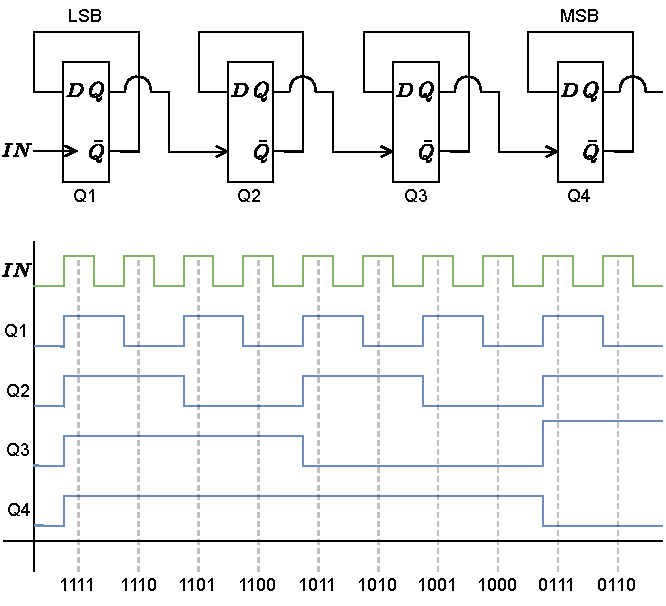
\includegraphics[width=0.75\textwidth]{includes/figures/defi_binaerzaehler.pdf}
    \end{center}
\end{defi}

\begin{defi}{Timer}
    Innerhalb eines Mikrocontrollers existieren verschiedenste Zähler, die mit einem (i. d. R. konfigurierbaren) Taktsignal betrieben werden.

    Wenn ein derartiger Zähler zum Auslösen von Ereignissen genutzt wird, spricht man von einem \emph{Timer}

    Timer lösen einen Interrupt aus.
\end{defi}

\begin{defi}{Timer Betriebsmodus}
    \begin{itemize}
        \item \emph{Capture Mode} (Stoppuhr):

              Aufgrund einer Taktflanke an einem Pin kann der Zähler gestartet werden und bei einer weiteren Flanke kann der aktuelle Zählwert in ein Register gespeichert werden.
              Wenn am Eingangspin eine Impulsfolge anliegt, kann man dann z. B. den Zeitabstand zwischen zwei Pulsen messen.
        \item \emph{Compare Mode} (Eieruhr):

              Wenn der Zähler einen speziellen Wert erreicht, kann er auf 0 zurückgesetzt werden.
        \item \emph{Output Mode}:

              Eine Erweiterung des \emph{Compare Mode}, bei dem beim Erreichen eines speziellen Wertes oder beim Rücksetzen bzw. Überlaufen des Zählers eine Ausgabeleitung gezielt verändert wird.
              Dadurch können z. B. PWM-Signale erzeugt werden.
    \end{itemize}
\end{defi}

\begin{defi}{Watchdog-Timer}
    Der \emph{Watchdog-Timer} ist wie ein Wachhund.

    Zum Reset des Systems wird er gestartet und zählt autonom regelmäßig hoch.

    Während eine Software läuft, muss der Watchdog Timer regelmäßig auf 0 zurückgesetzt werden.
    Dies geschieht i. d. R. an einer zentralen Stelle in der Software.

    Falls der Watchdog-Timer zu lange nicht \enquote{gefüttert} wurde, wird ein System-Reset ausgeführt.
    Meist passiert das nur, wenn die Software abgestürzt ist.
\end{defi}

\begin{bonus}{Timer im MSP432}
    \begin{itemize}
        \item \texttt{ACLK} (Auxiliary Clock)
        \item \texttt{MCLK} (Main (CPU) Clock)
        \item \texttt{HSMCLK} (Highspeed Subsystem Main Clock)
        \item \texttt{SMCLK} (Subsystem Main Clock)
    \end{itemize}

    Bei einem System-Reset werden alle Timer von dem DCO auf 3MHz eingestellt.

    Es lässt sich ebenfalls ein Vielfaches von 3MHz als Frequenz einstellen.
    Die Maximalfrequenz liegt bei 48MHz.
\end{bonus}

\begin{defi}{Timer A}
    Der \emph{Timer\_A} ist ein 16-bit Zähler, der von unterschiedlichen Taktsignalen gespeist werden kann.
    Der MSP432 besitzt 4 \texttt{Timer\_A} Module.

    Jeder Timer besitzt ein \emph{Capture and Compare Register (CCR)}.
    Zusätzlich lässt sich einer von 7 Output-Modi einstellen:

    \begin{center}
        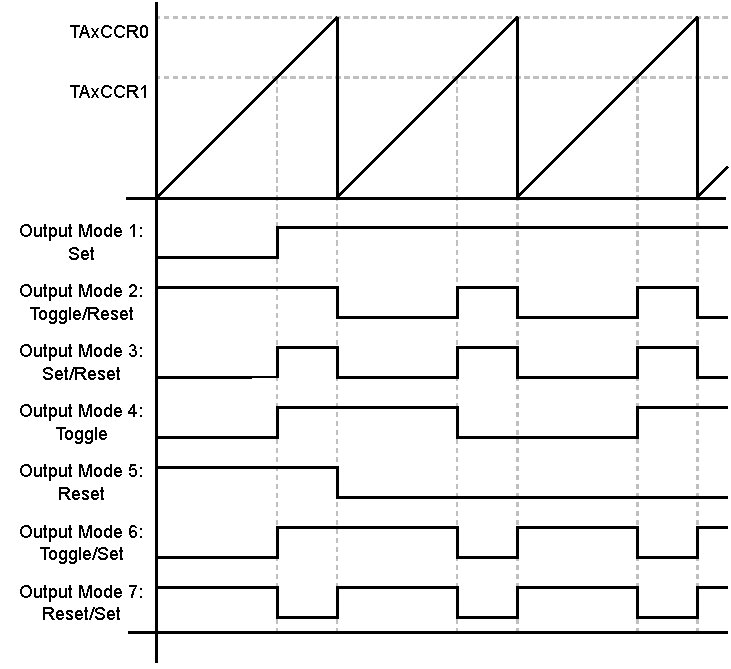
\includegraphics[width=0.65\textwidth]{includes/figures/defi_timer_a.pdf}
    \end{center}
\end{defi}

\begin{defi}{PWM}
    \emph{Pulse Width Modulation (PWM)}-Signale erstellen bei konstanter Frequenz unterschiedlich lange Zeiten im High- und Low-Zustand.

    Das Verhältnis der Einschalt- zur Gesamtdauer einer Schwingung nennt man Tastverhältnis und ist als $\nicefrac{t_1}{T}$ definiert.

    OWM-Signale werden genutzt zum:
    \begin{itemize}
        \item Steuern von Motoren
        \item Dimmen von Lampen
        \item Regeln von Spannungen in Netzteilen
    \end{itemize}
\end{defi}

\begin{example}{PWM}
    Erzeuge ein PWM-Signal von 100Hz und einem Tastverhältnis von 20\%.

    Der Timer TA0 wird mit 3MHz betrieben:

    \[
        \text{TA0CCR0} = \frac{\SI{3}{\mega\hertz}}{\SI{100}{\hertz}} = \num{30000}
    \]

    Wir brauchen ein Tastverhältnis von 20\%:

    \[
        \text{TA0CCR0} = (1 - \text{Tastverhältnis}) \cdot \text{TA0CCR0} = 0.8 \cdot \num{30000} = \num{24000}
    \]

    Wenn wir \texttt{CCR1} z. B. mit \texttt{Set/Reset (Mode 3)} und den errechneten Grenzen betreiben, erhalten wir das gewünschte Ergebnis.

    \begin{center}
        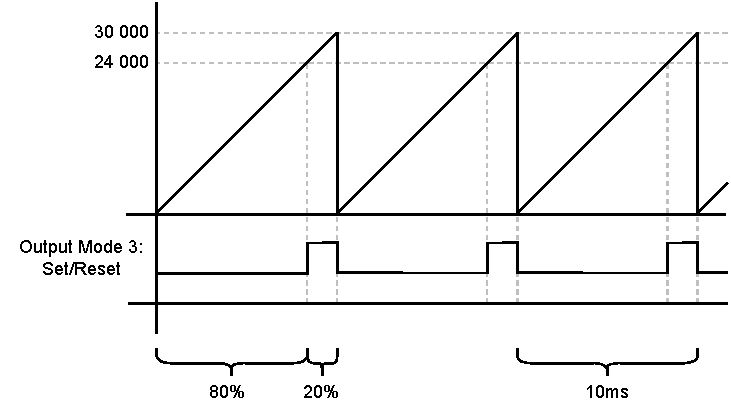
\includegraphics[width=0.65\textwidth]{includes/figures/example_timer_a.pdf}
    \end{center}
\end{example}

\begin{bonus}{MSP432 Implementierung}
    Um einen GPIO-Pin als \texttt{Timer\_A} zu verwenden, sind neben dem \texttt{PxDIR} Register \texttt{PxSEL0} auf \texttt{1} und \texttt{PxSEL1} auf \texttt{0} zu setzten.
\end{bonus}